\chapter{Resultados}
\label{resultados}

\section{Dados Obtidos}
Os dados armazenados foram extraídos do banco de dados em um arquivo no formato CSV, \emph{Comma Separated Values}(Valores Separados por Virgula), o arquivo possui as mesmas informações apresentadas na seção \ref{experimento} e contém um total de 462.065 linhas, a figura \ref{fig:csv_example} ilustra as primeiras linhas do arquivo CSV. A partir deste arquivo CSV, foi gerado onze novos arquivos, um para cada dispositivo Tx, que possui apenas o identificador do pacote, o horário da transmissão e quais tentativas de transmissão foram bem sucedidas, a figura \ref{fig:second_csv_example} ilustra este arquivo, no qual o número ``1'' significa uma tentativa de transmissão bem sucedida e o número ``0'' significa que não foi recebido a mensagem com daquela modulação com aquele identificado.


\begin{figure}[h]
    \centering
    \begin{subfigure}{.4\textwidth}
        \centering
        \caption{Exemplo das Colunas do Arquivo CSV.}
        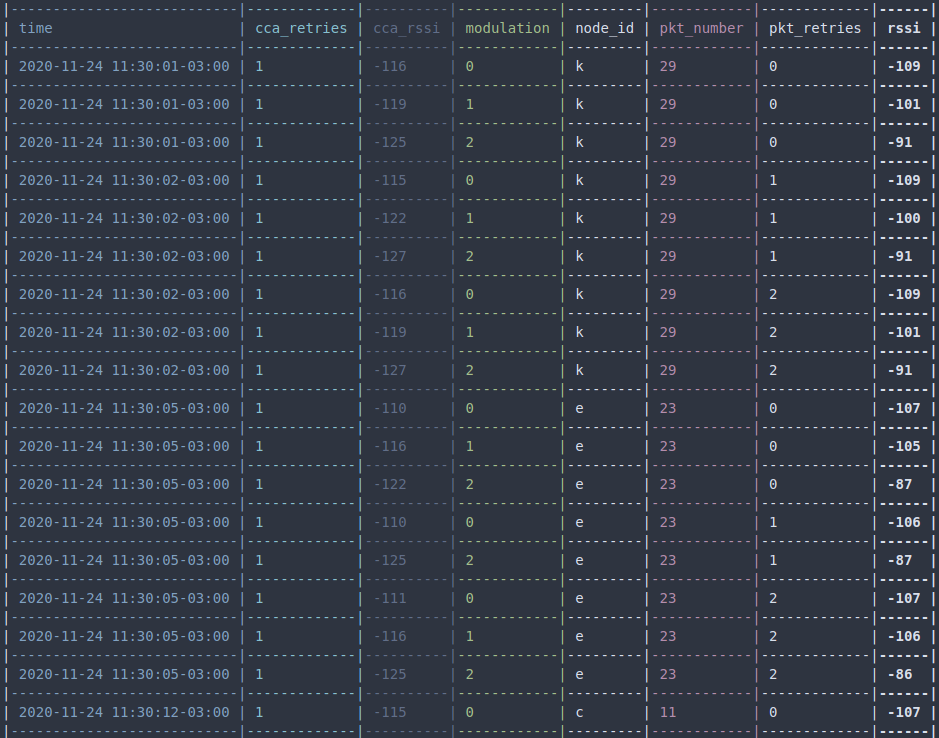
\includegraphics[width=\textwidth]{./sections/textual/chapters/images/csv_example.png}
        \label{fig:csv_example}
    \end{subfigure}
    \begin{subfigure}{.4\textwidth}
        \centering
        \caption{Exemplo do Arquivo com as Tentativas de Transmissão.}
        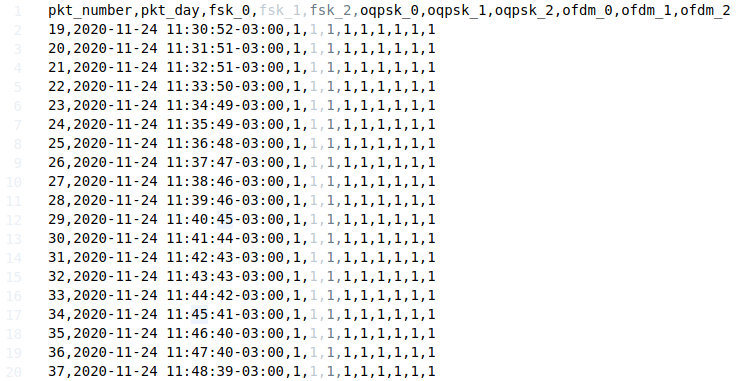
\includegraphics[width=\textwidth]{./sections/textual/chapters/images/second_csv_example.png}
        \label{fig:second_csv_example}
    \end{subfigure}
    \caption{Dados do experimento.}
    \label{fig:test}
\end{figure}

Todos os arquivos CSV e scripts utilizados para a analise de dados estão disponíveis no repositório \cite{wisun-traces}.

\section{Valores de PDR}
A partir dos onze arquivos com as tentativas de transmissão, foi calculado o PDR de cada cada modulação, para cada um dos dispositivos Tx em cada uma das três transmissões realizadas. Na tabela \ref{table:pdr} estão detalhados os valores de PDR para cada dispositivo, modulação e transmissão. Os dispositivos ``D'' e ``H'' foram posicionados no primeiro piso, os dispositivos ``A'', ``B'' e ``C'' foram posicionados no segundo piso, os grupos formados pelos dispositivos ``E'', ``F'' e ``G'' e ``I'', ``J'' e ``K'' foram posicionados no terceiro e quarto piso do prédio, respectivamente.

Importante destacar, as mensagens enviadas pela modulação SUN-OFDM pelo dispositivo ``H'' possui um menor valor de PDR do que os dispositivos próximos, mesmo estando no proximo ao Rx, provavelmente devido a efeitos de sombreamento, no qual as diversas replicas de sinais propagados por múltiplos caminhos até o receptor realizem uma soma destrutiva proxima ao receptor causando problemas na recepção de sinal, este efeito é perceptível também em outros dispositivos. No dispositivo ``K'' é observado que os valores de PDR são maiores que os outros dispositivos do mesmo andar, neste caso, provavelmente, o fato do dispositivo Tx está posicionado em uma sala diretamente acima do receptor facilitou a propagação do sinal criando, proximo ao receptor, uma área que os sinais que percorreram múltiplos caminhos onde o sinal tenha uma melhor recepção.

\begin{table}[ht]
    \centering
    \caption{Valores de PDR para cada dispositivo.}
    \begin{tabular}{|c|c|c|c|c|c|c|c|c|c|}
        \hline
        ID                     & \multicolumn{3}{c|}{\textbf{SUN-FSK}} & \multicolumn{3}{c|}{\textbf{SUN-OQPSK}} & \multicolumn{3}{c|}{\textbf{SUN-OFDM}}                                                                                                       \\ \cline{2-10}
                               & \textbf{P$_1$}                        & \textbf{P$_2$}                          & \textbf{P$_3$}                         & \textbf{P$_1$} & \textbf{P$_2$} & \textbf{P$_3$} & \textbf{P$_1$} & \textbf{P$_2$} & \textbf{P$_3$} \\ \hline
        \texttt{D}             & 80.39                                 & 78.71                                   & 80.17                                  & 99.20          & 99.17          & 99.17          & 99.21          & 99.21          & 99.21          \\ \hline
        \texttt{H}             & 80.86                                 & 78.67                                   & 80.97                                  & 99.21          & 99.21          & 99.21          & 45.12          & 45.19          & 45.31          \\ \hline
        \texttt{A}             & 99.17                                 & 99.15                                   & 99.15                                  & 99.20          & 99.21          & 99.21          & 99.15          & 99.15          & 99.18          \\ \hline
        \texttt{B}             & 98.08                                 & 97.93                                   & 98.10                                  & 97.85          & 98.32          & 98.44          & 99.04          & 98.94          & 99.02          \\ \hline
        \texttt{C}             & 28.11                                 & 20.21                                   & 28.17                                  & 99.07          & 98.95          & 99.01          & 96.40          & 96.40          & 96.37          \\ \hline
        \texttt{E}             & 69.71                                 & 63.88                                   & 69.71                                  & 99.20          & 99.21          & 99.21          & 98.53          & 98.60          & 98.58          \\ \hline
        \texttt{F}             & 86.56                                 & 83.35                                   & 85.67                                  & 99.21          & 99.21          & 99.18          & 88.12          & 88.23          & 88.17          \\ \hline
        \texttt{G}             & 0.18                                  & 0.15                                    & 0.15                                   & 76.59          & 76.45          & 75.82          & 0.07           & 0.07           & 0.15           \\ \hline
        \texttt{I}             & 6.10                                  & 5.77                                    & 6.12                                   & 57.90          & 57.92          & 58.36          & 0.00           & 0.00           & 0.00           \\ \hline
        \texttt{J}             & 0.01                                  & 0.01                                    & 0.00                                   & 25.02          & 25.33          & 24.86          & 1.78           & 1.94           & 1.83           \\ \hline
        \texttt{K}             & 97.56                                 & 97.36                                   & 97.53                                  & 98.15          & 98.15          & 98.16          & 56.75          & 57.29          & 56.89          \\ \hline
        \textbf{Média}         & 58.79                                 & 56.83                                   & 58.70                                  & 86.42          & 86.47          & 86.42          & 62.20          & 62.28          & 62.25          \\ \hline
        \textbf{Desvio Padrão} & 41.39                                 & 41.50                                   & 41.32                                  & 24.34          & 24.28          & 24.39          & 43.54          & 43.51          & 43.52          \\ \hline
    \end{tabular}
    \label{table:pdr}
\end{table}

Observando os dados da figura \ref{fig:pdr_andar} a modulação SUN-OQPSK se destaca em relação as outras. Como apresentado na seção \ref{padrõesSF} as modulações SUN-OQPSK e SUN-OFDM possuem maior robustez a interferências e efeitos negativos da propagação por múltiplos caminhos, porém, como apresentado na tabela \ref{table:config}, a modulação SUN-OQPSK possui maior potência de transmissão comparado ao SUN-OFDM, devido a limitações de \emph{hardware}. Logo, é de se esperar que a modulação SUN-OQPSK possua melhores valores de PDR.


\begin{figure}[ht!]
    \centering
    \begin{subfigure}{.4\textwidth}
        \centering
        \caption{Primeiro Piso.}
        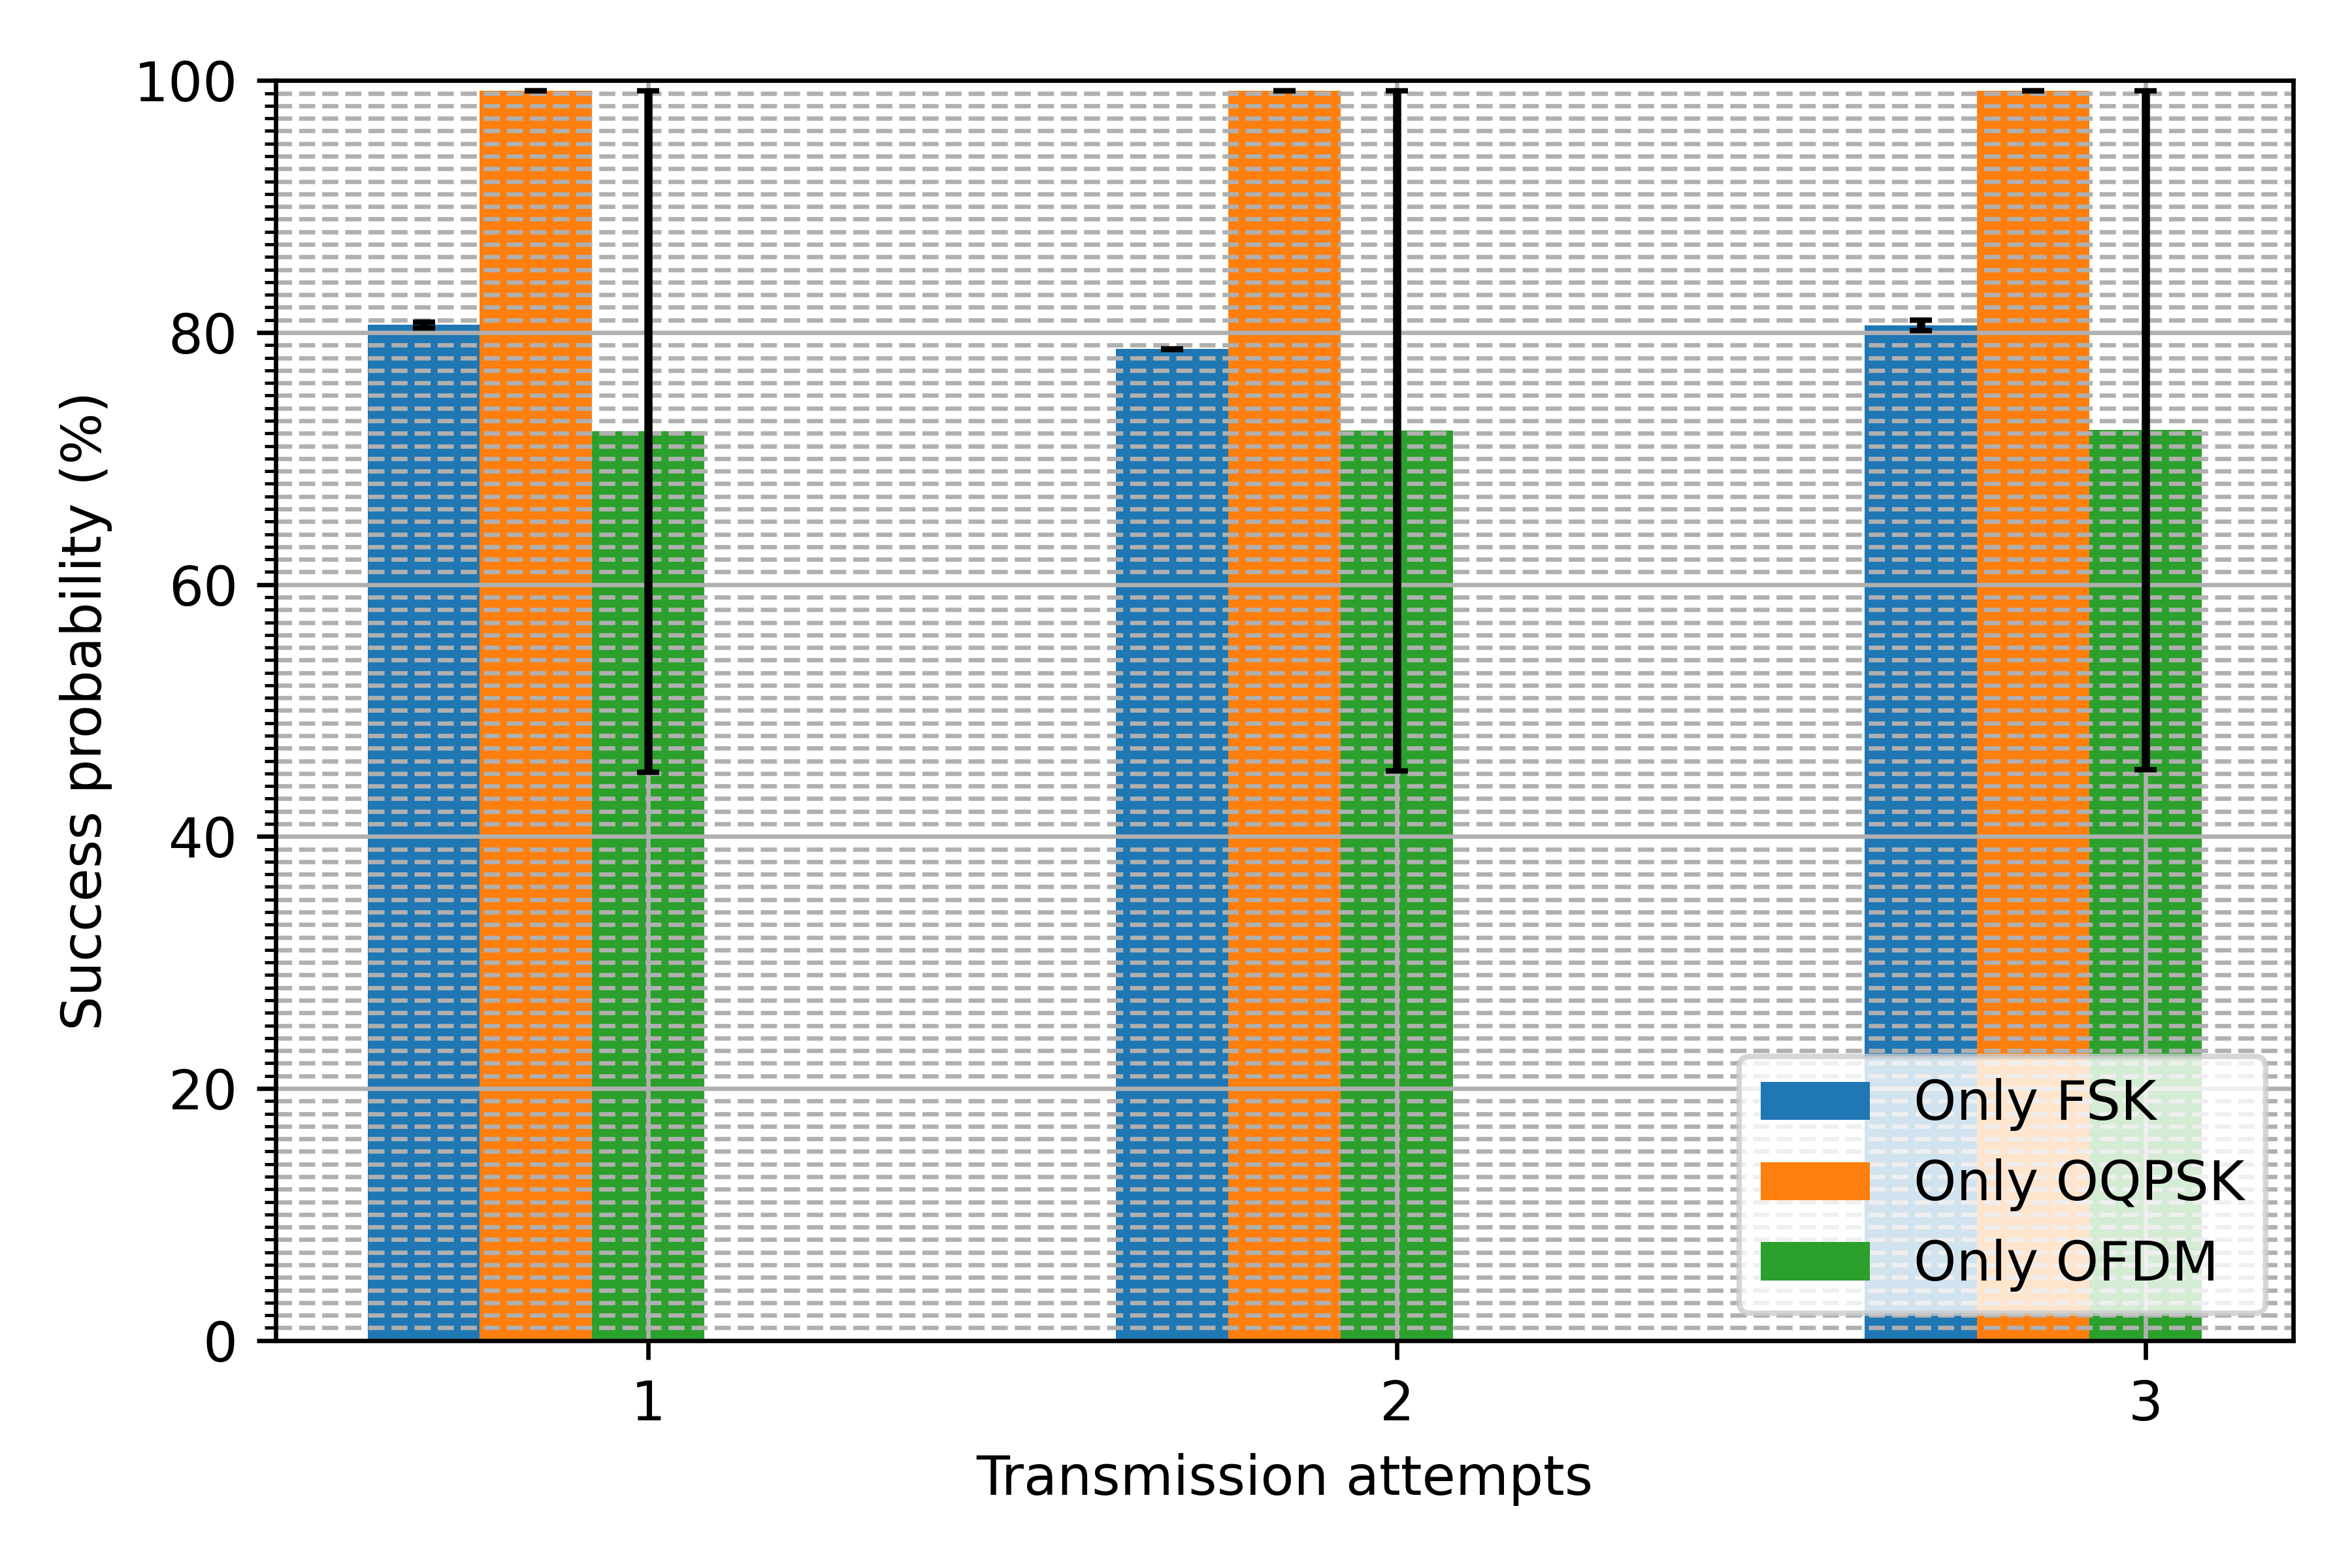
\includegraphics[width=\textwidth]{./sections/textual/chapters/images/mod_1_floor.png}
        \label{fig:piso1}
    \end{subfigure}
    \begin{subfigure}{.4\textwidth}
        \centering
        \caption{Segundo Piso.}
        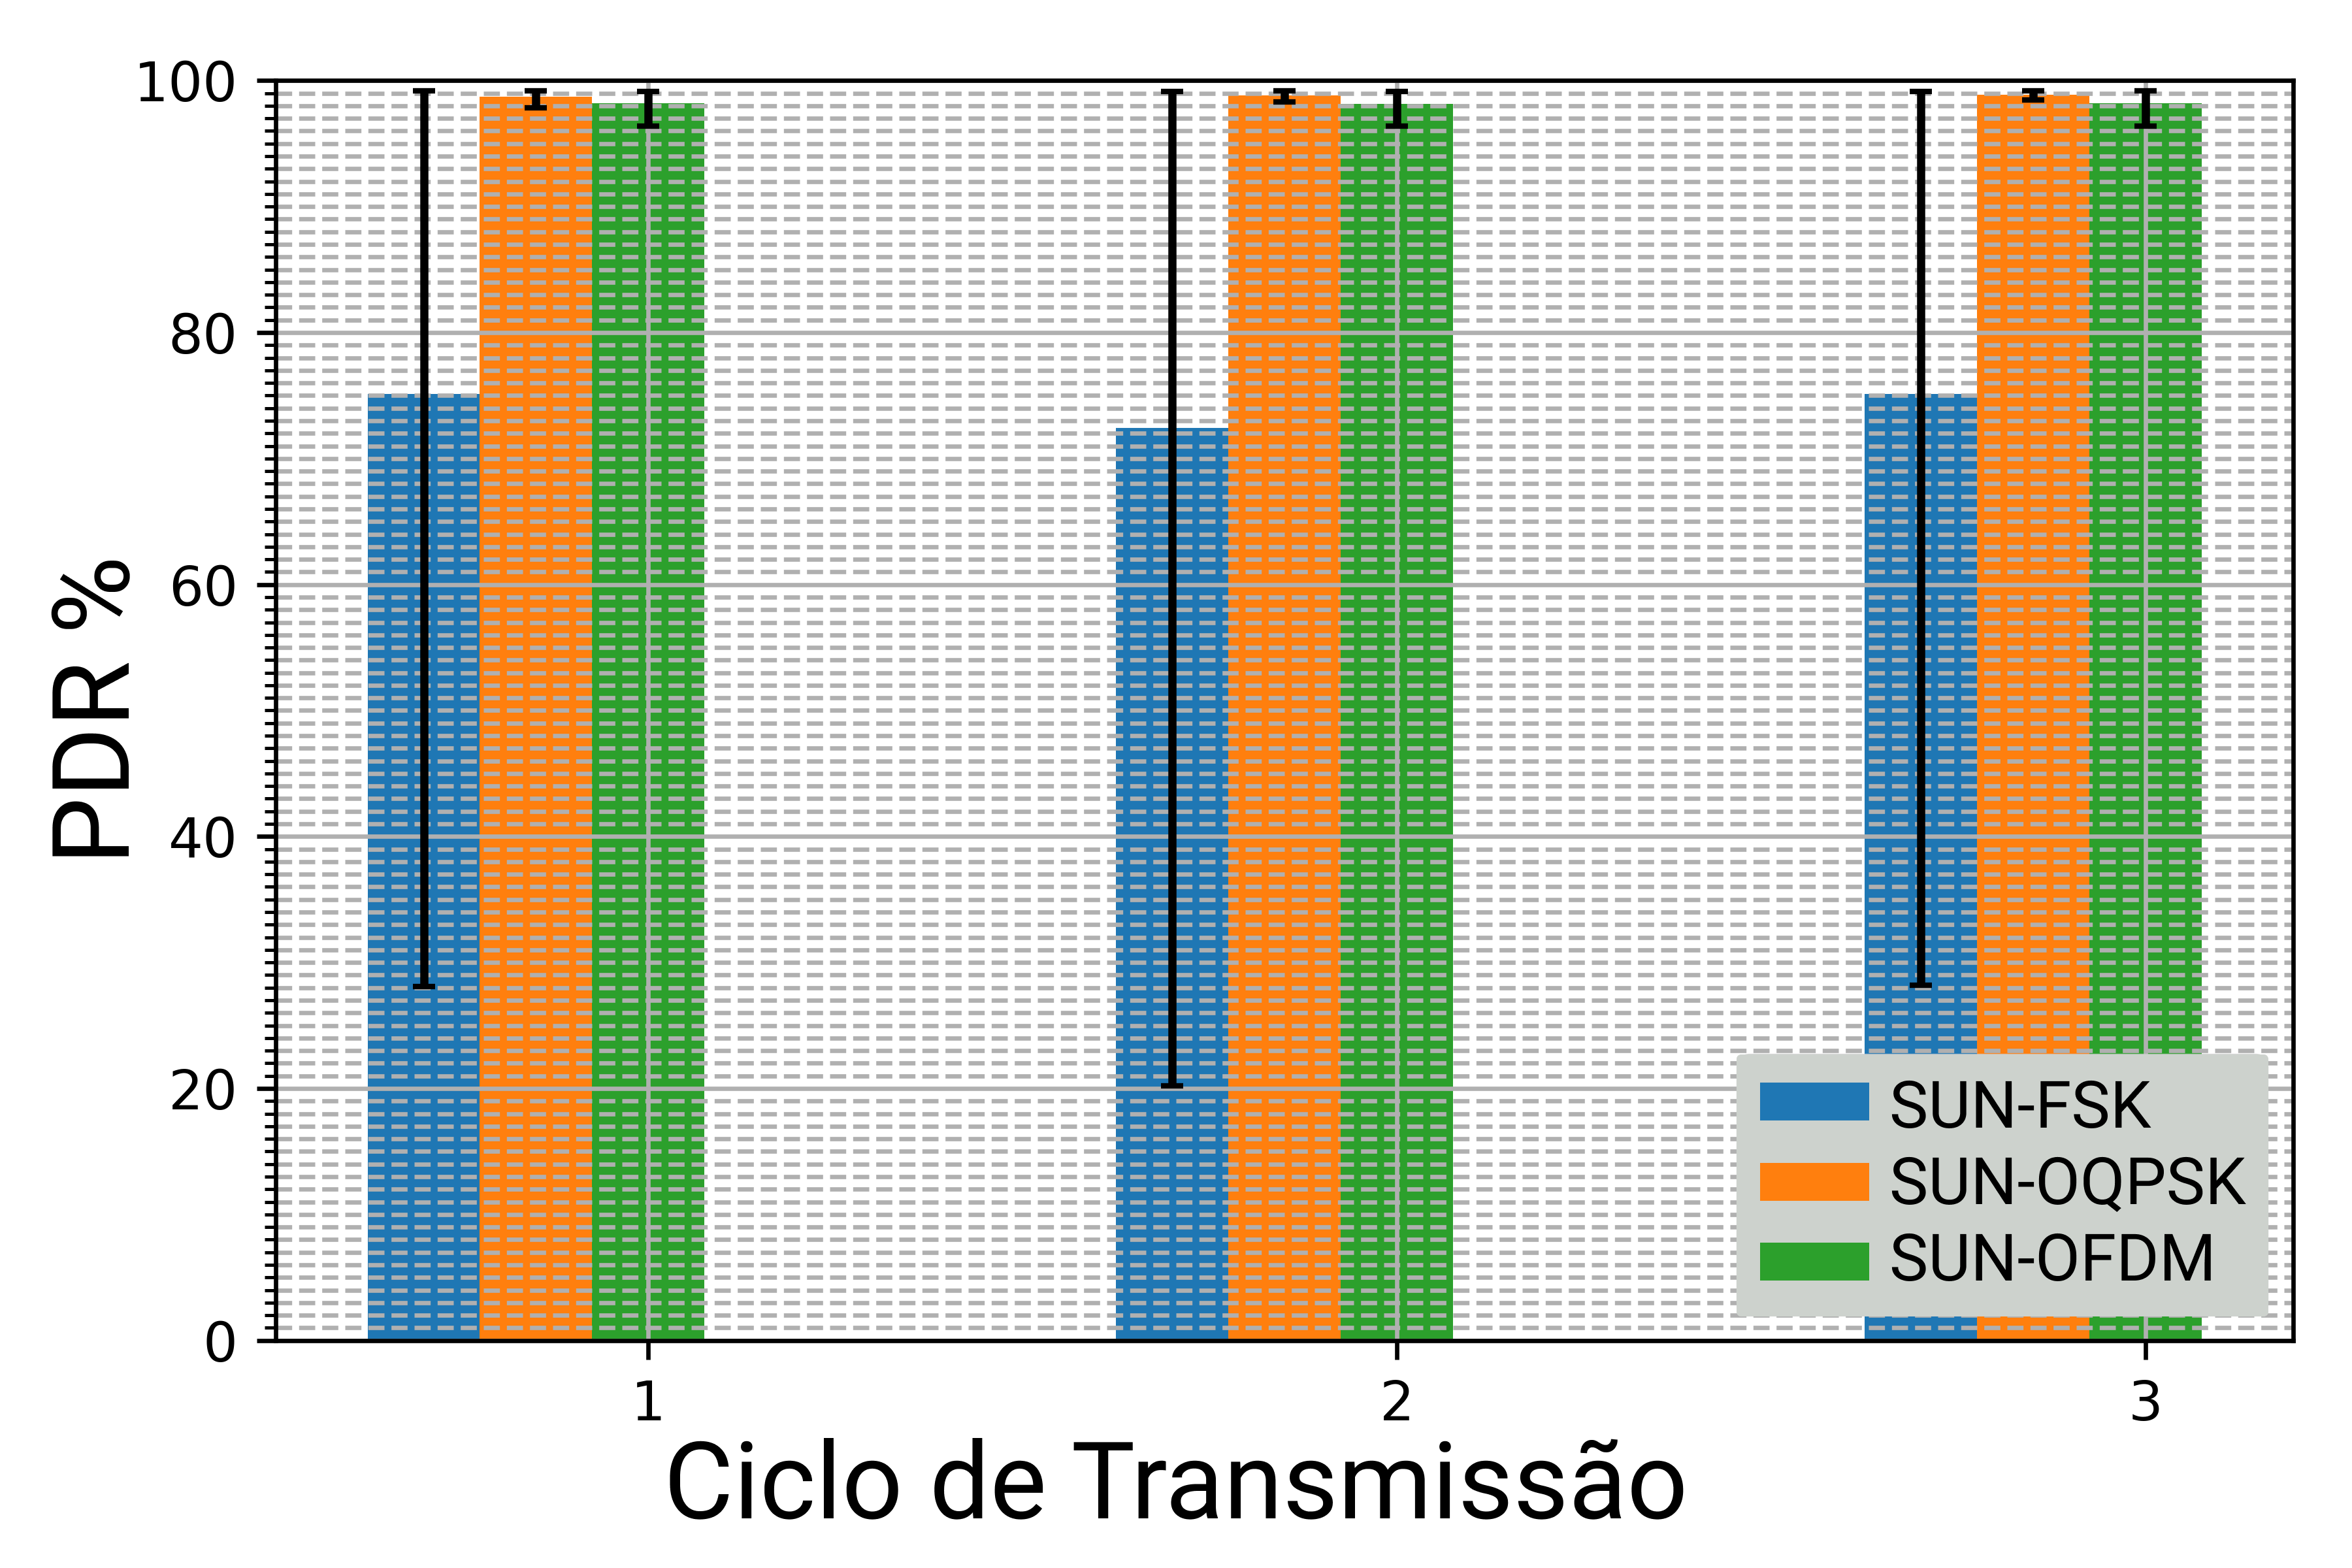
\includegraphics[width=\textwidth]{./sections/textual/chapters/images/mod_2_floor.png}
        \label{fig:piso2}
    \end{subfigure}
    \begin{subfigure}{.4\textwidth}
        \centering
        \caption{Terceiro Piso.}
        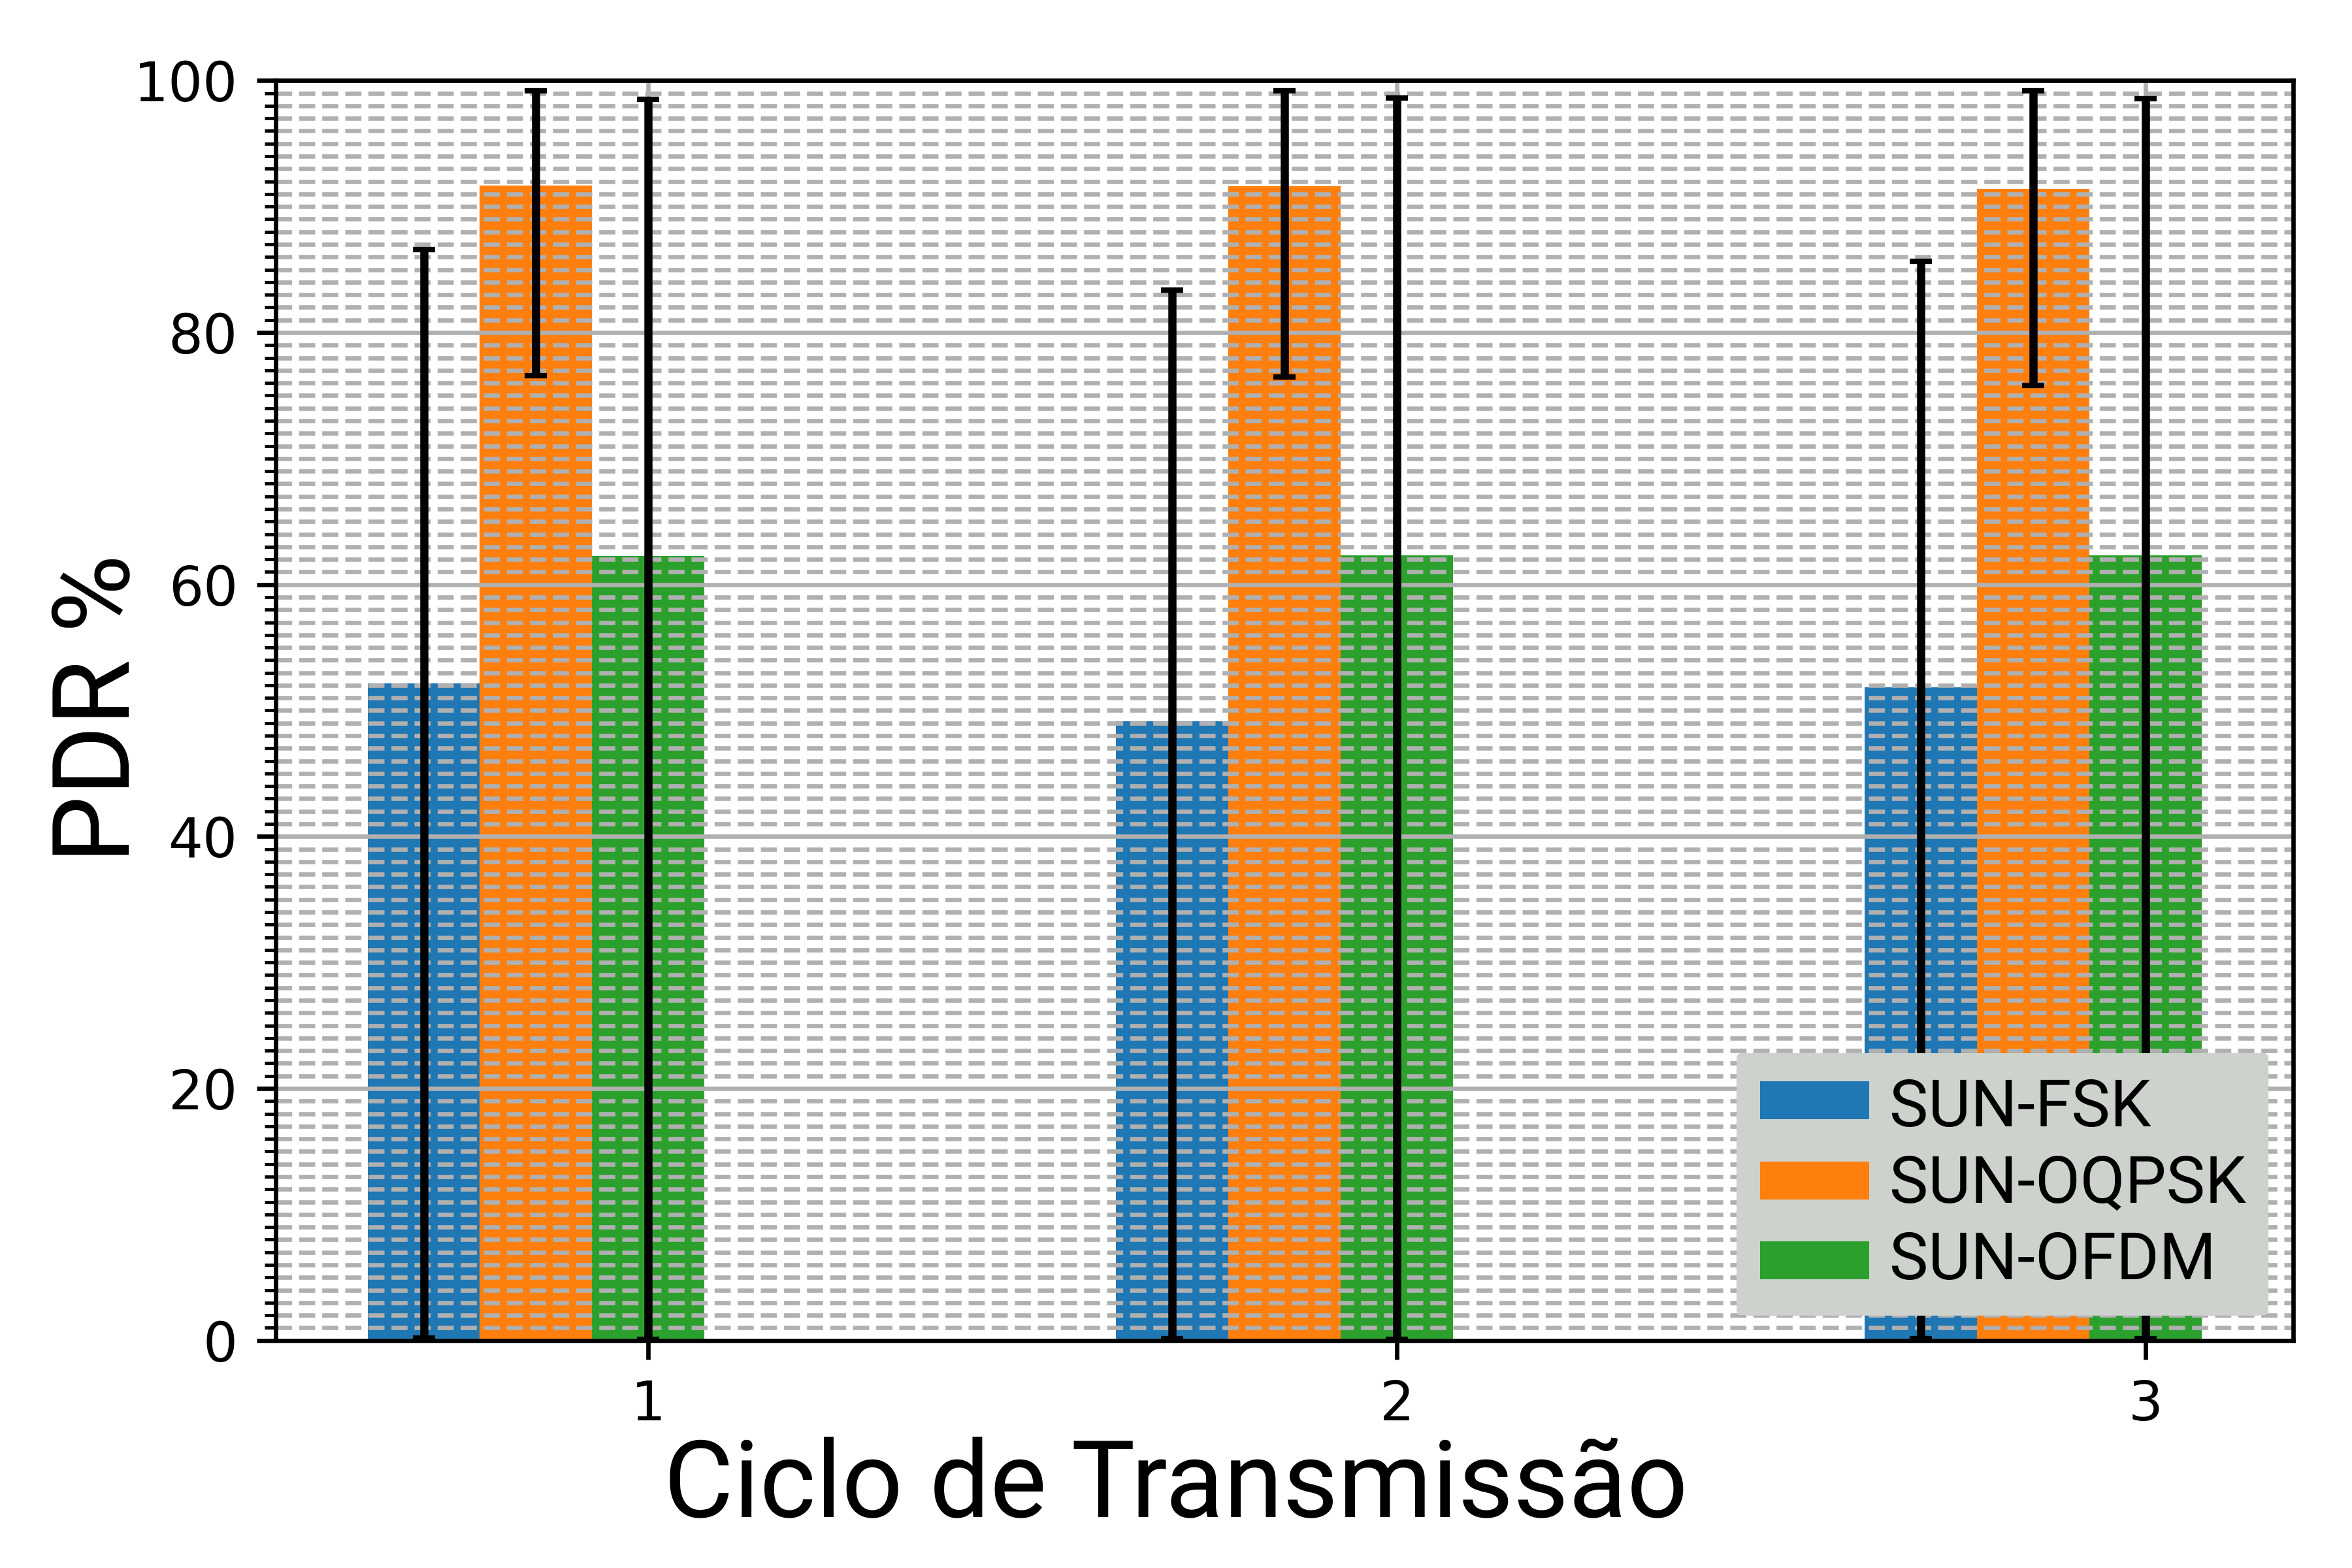
\includegraphics[width=\textwidth]{./sections/textual/chapters/images/mod_3_floor.png}
        \label{fig:piso3}
    \end{subfigure}
    \begin{subfigure}{.4\textwidth}
        \centering
        \caption{Quarto Piso.}
        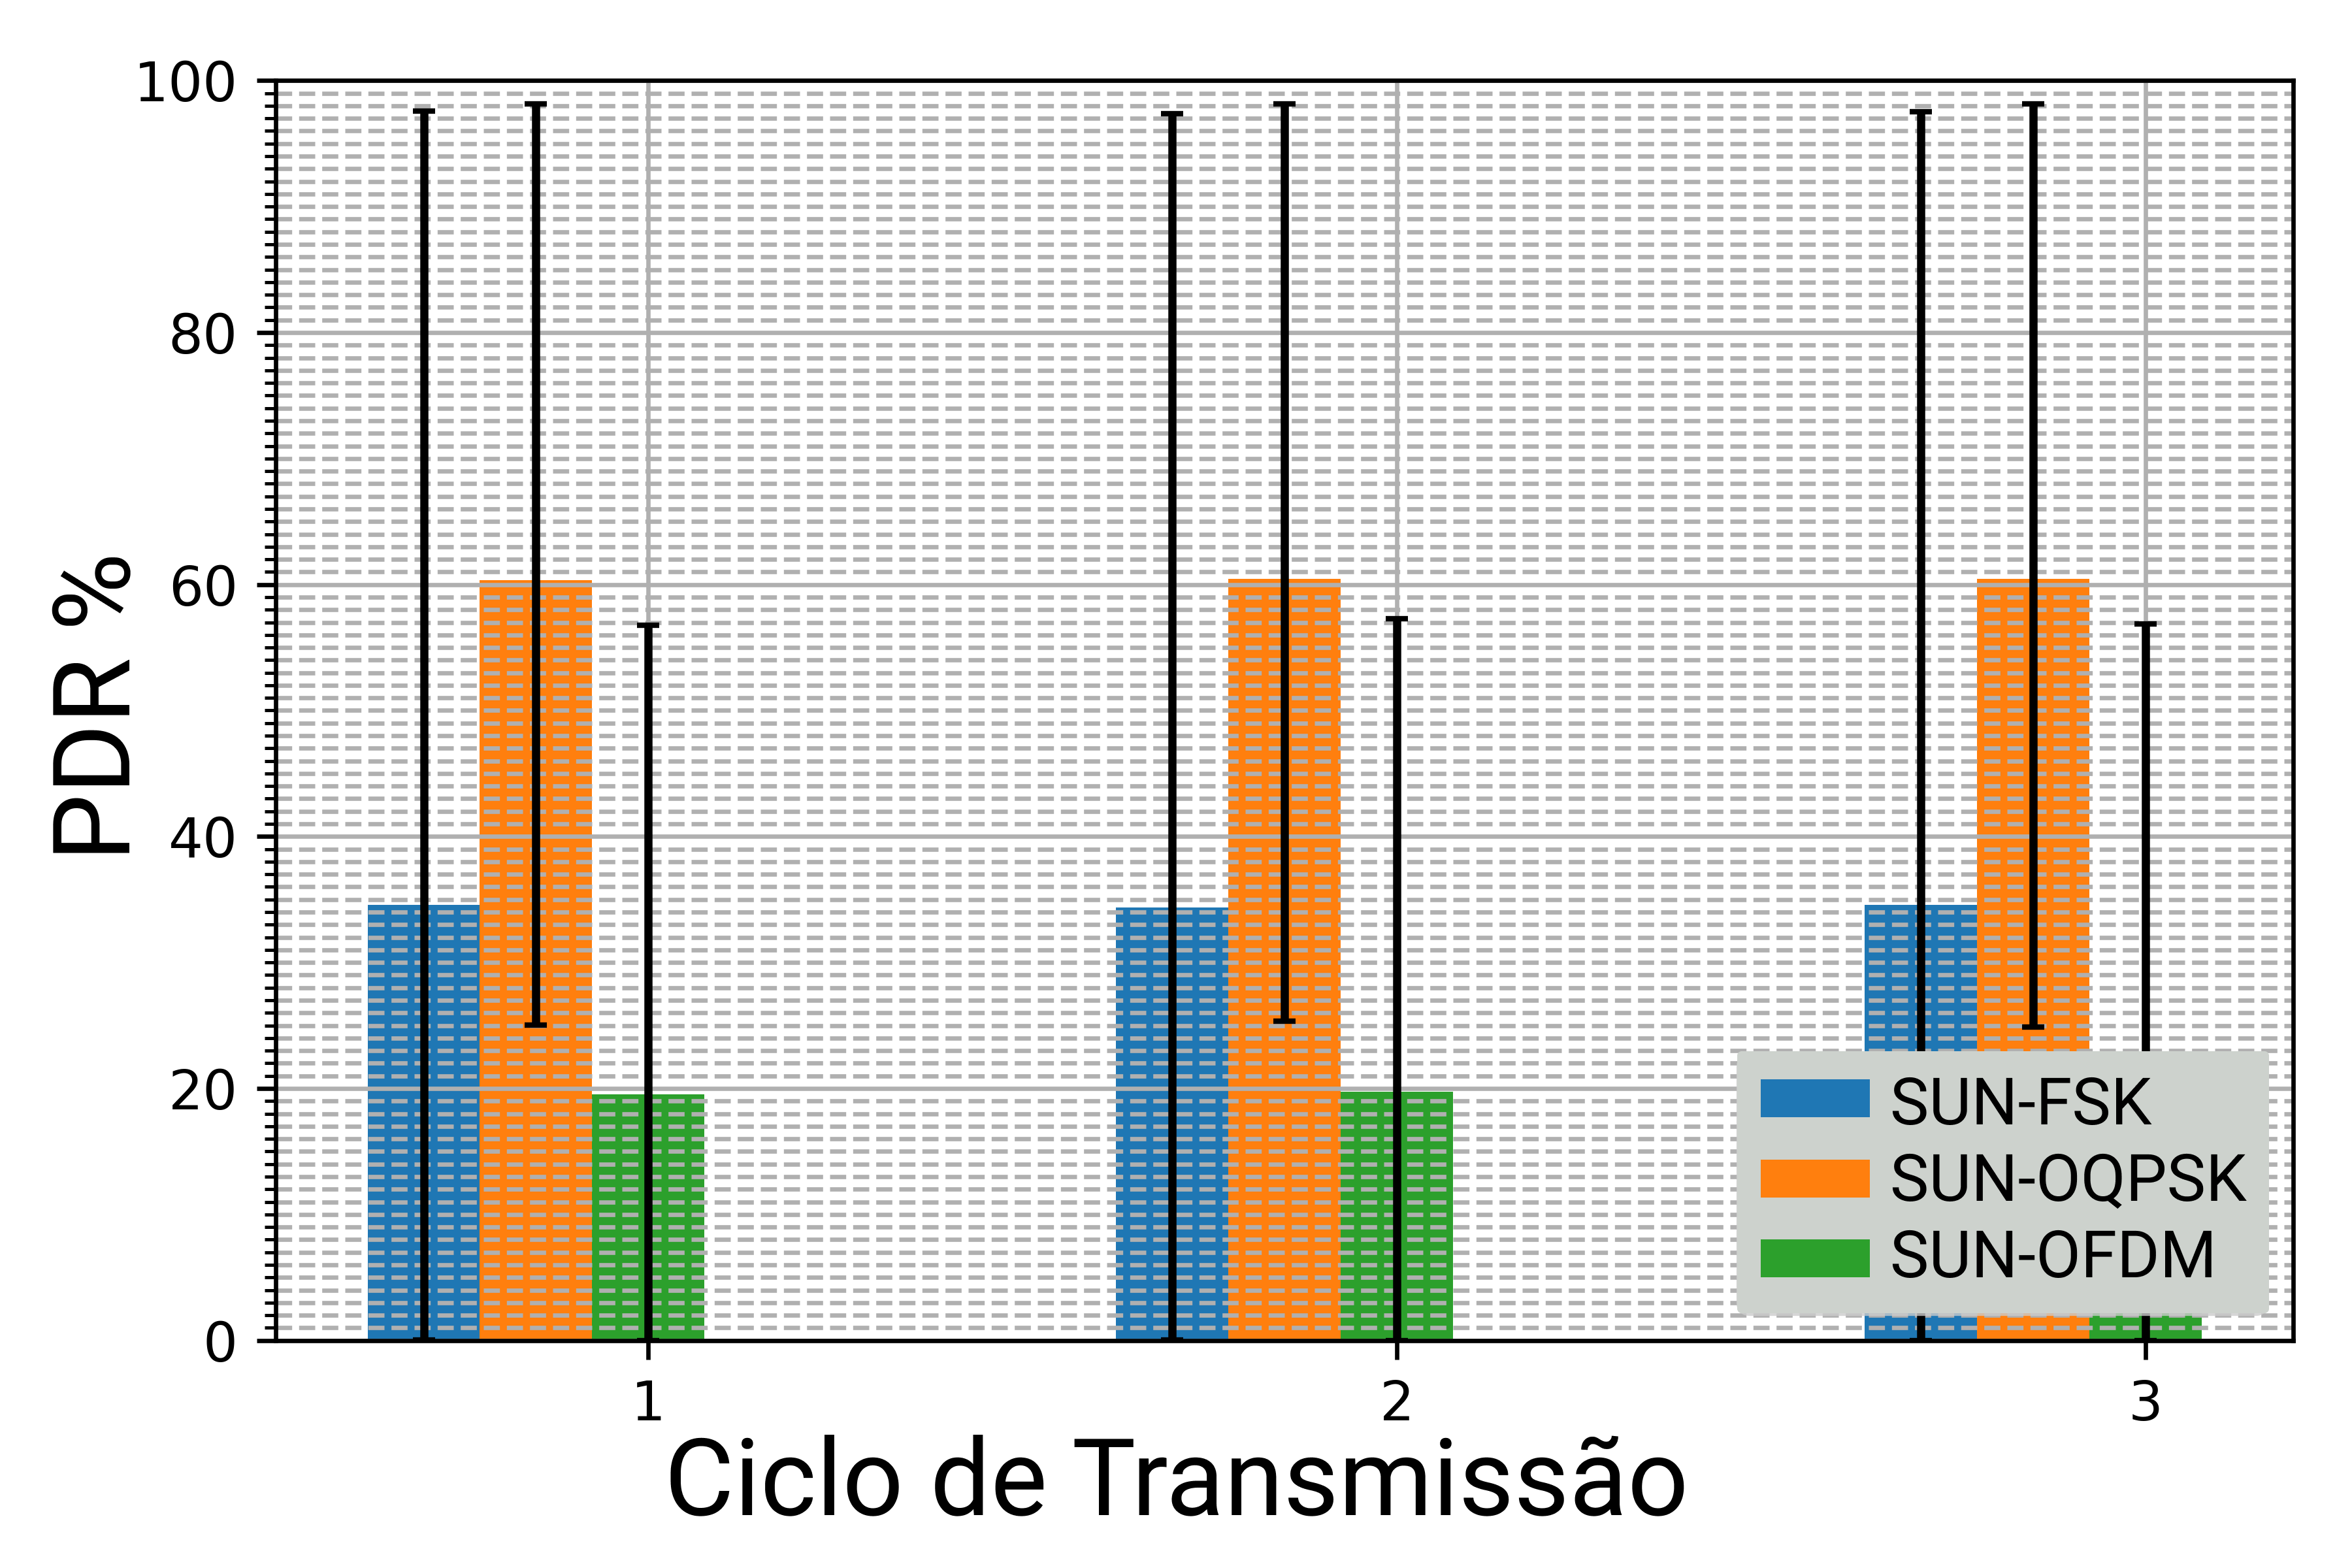
\includegraphics[width=\textwidth]{./sections/textual/chapters/images/mod_4_floor.png}
        \label{fig:piso4}
    \end{subfigure}
    \caption{Valores de PDR para cada piso.}
    \label{fig:pdr_andar}
\end{figure}


\todo{Fazer a analise de RSSI e CCA}